\documentclass{article} % For LaTeX2e
\usepackage{nips15submit_e,times}
\usepackage{amsmath}
\usepackage{hyperref}
\usepackage{url}
\usepackage{graphicx}
%\documentstyle[nips14submit_09,times,art10]{article} % For LaTeX 2.09


\title{Approximately Bayesian Demixing with Neural Networks \\ David Halpern}


\author{
David Halpern\\
Department of Psychology\\
New York University\\
\texttt{david.halpern@nyu.edu} \\
}

\newcommand{\fix}{\marginpar{FIX}}
\newcommand{\new}{\marginpar{NEW}}

\nipsfinalcopy % camera-ready version

\begin{document}


\maketitle


\section{Introduction}
Sensory brain areas are often tasked with figuring out information about the multitude of stimuli out in the world. However, these areas must solve this problem using only the spikes from upstream neurons. Neurophysiological evidence suggests that, in many brain regions, neural responses to multiple simultaneously-presented stimuli can be accurately described as sums of the responses to the stimuli presented by themselves (e.g. IT \cite{Zoccolan07112007}, V1 \cite{Busse2009}, MT \cite{Britten15061999}). This can present problems when it is unclear whether just one stimulus is being presented at a high contrast or two at a lower contrast. 
\begin{figure}[h]
\centering
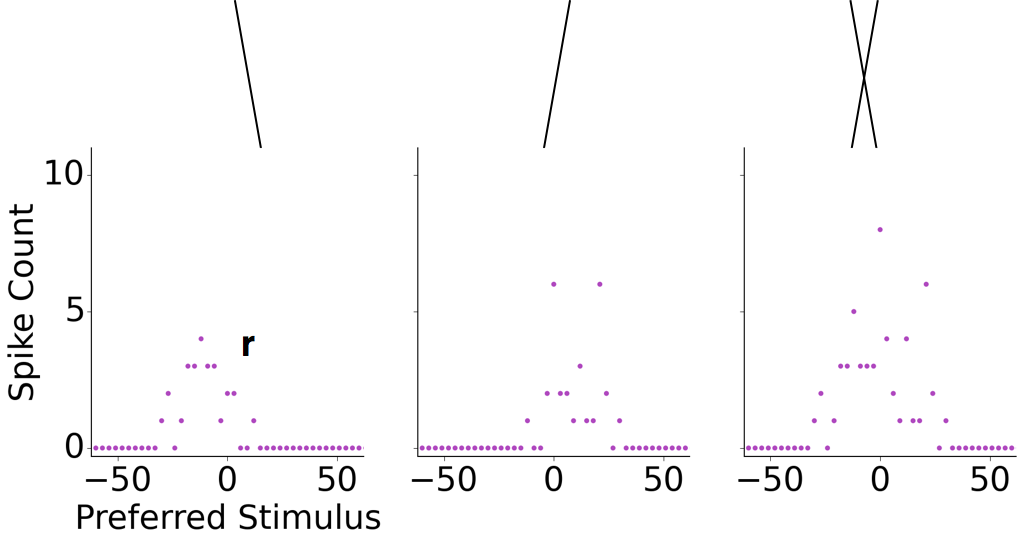
\includegraphics[width = \textwidth]{Neural_Response.png}
\caption{Responses of a population of orientation-tuned neurons to two stimuli presented individually and together}
\label{Neural_Response}
\end{figure}
For example, Figure \ref{Neural_Response} shows the responses of orientation-tuned neurons (such as those in V1) to isolated and simultaneously presented orientations. The downstream neurons must take these mixed stimulus responses and extract information about the individual stimuli. We call this the "demixing" problem. In the following, we investigate how the brain might solve this problem.
\\
If we have a probability model for how the neural responses were generated, the posterior mean gives the best possible estimator of the generating stimulus, given the information from the neural responses. In addition, the posterior gives not only an estimator but the probability of any generating stimulus (within the support of the probability model). This means that if downstream neurons could compute the posterior over stimuli, they would also be able to compute the uncertainty of our estimate or other quantities of interest (like the probability that a line has an orientation greater than 90$^{\circ}$). Bayesian decision theory requires the probability of various outcomes to allow an agent to make optimal decisions. In fact, many studies of perception and cognition suggest that human subjects can well approximate the optimal Bayesian solution to many problems /cite{?}. Bot the theoretical optimality and psychophysical evidence have led many computational neuroscientists to come up with neurally plausible implementations of Bayesian inference (i.e. \cite{Ma2006}). In the past, this program of research has generally taken on only simple cases and has not led to very general inference algorithms that can be widely applied throughout the brain. It is unclear whether this is a promising direction since the posterior is not analytic in all but toy problems or even computationally tractable in high-dimensional cases. There has been a lot of research in machine learning and statistics on how to tractably approximate Bayesian inference and some research on whether neurons could apply these solutions \cite{?}. However, these solutions often still require neurons to do highly biologically implausible computations. 
One alternative to this approach is to look at the literature on artificial neural networks. Here, they use units that locally do only biologically plausible computations (like linear combinations with pointwise nonlinearities) to do function approximation. When layers of nonlinearities are stacked on top of each other and the weights are properly trained, these networks can well approximate highly complex functions. The past few years have seen a resurgence of these techniques in the machine learning world for learning functions in complex tasks like object and speech recognition \cite{?}. In the following, we attempt to approximate the function from incoming spike trains to estimates of the generating stimuli using small layered networks of these types of neurons and compare that to the optimal posterior mean estimate.

\section{Methods}
In order to test the performance of the neural networks, we generated stimuli according to the following statistical model. We used two stimuli for all but the last experiment when only one was used. $s_1$ was drawn discrete uniform distribution over the interval [-60, 60]. $s_2$ was then drawn from the interval [$s_1$, 60]. Finally, we generated a neural response with Poisson noise and tuning curves were given by linear combinations of the responses to each individual input. In notation:
\begin{equation}
	\mathbf{r} = \text{Poisson}(\sum_i g_i \mathbf{f}(s_i))
\end{equation}
where $\mathbf{r}$ is the vector of spike counts on a particular trial, $\mathbf{f}$ is the vector of tuning curves for individual stimuli, $g_i$ is the gain for the $i$th stimulus and $s_i$ is the orientation of the $i$th stimulus. Gain here can be thought of as being the neural representation of the contrast of the stimulus (although could be modulated by many other things such as attention).
Each tuning curve is given by
\begin{equation}
	f_i = e^\frac{(s - s_{\text{pref}_i})^2}{2 \sigma_{tc}^2}
\end{equation}
\begin{figure}[h]
\centering
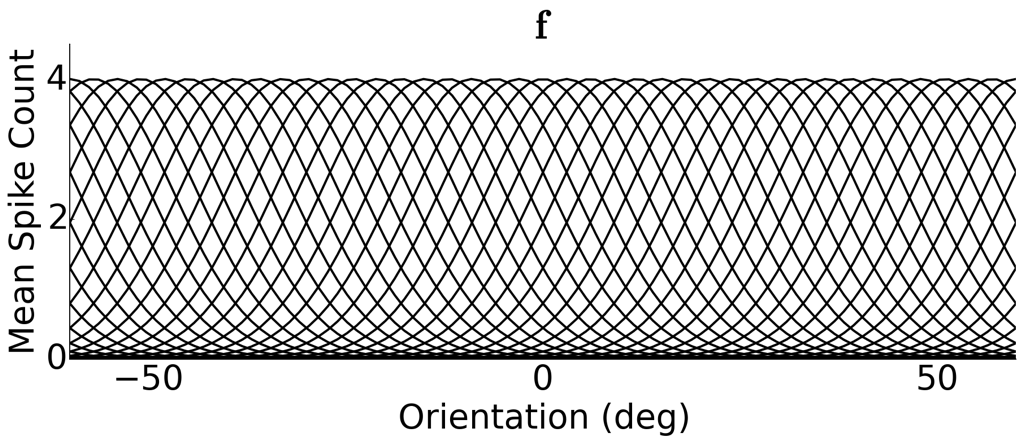
\includegraphics[width = \textwidth]{Tuning_Curves.png}
\caption{Mean firing rate of every neuron in the input population as a function of stimulus input}
\end{figure}
\\
All of the $s_{\text{pref}_i}$ were evenly tiled over [-90, 90]. This was larger than the range of possible stimuli in order to mitigate edge effects. In our simulations we used 61 neurons and $\sigma_{tc}$ was set to 10.
\\
\\
We computed the posterior mean on every trial in order to have a baseline for comparison with the networks. We computed this using a grid approximation where we computed the unnormalized posterior at all the possible combinations of $s_1$ and $s_2$.
\\
\\
Throughout, we investigate the performance of a three layer nonlinear network with an input layer, a hidden layer and an output layer (which produces the estimates). The input layer consisted of the 61 neurons described above. The neural network then included a hidden layer with 20 units which are fully connected to all of the input units. The activation function for the hidden units is given by a linear combination of the inputs followed by a pointwise nonlinearity. Again, in notation:
\begin{equation}
	\mathbf{r}_{\text{hid}} = \sigma(\mathbf{Wr + b})
\end{equation}
Where $\mathbf{r}_{\text{hid}}$ is the vector of activations, $W$ is the matrix of weights and $b$ is a vector of bias terms. For the nonlinearity, we used Rectified Linear Units \cite{NairH10} which are defined as:
\begin{equation}
	\sigma(x) = \max(0, x)
\end{equation}
We used this nonlinearity both due to it's biological plausibility (since biological neurons cannot have negative firing rates) and due to it's success within the machine learning community \cite{Maas2013}.
Finally, the network outputs (estimates of $\mathbf{s}$) were linear combinations of the hidden unit activations,  
\begin{equation}
	\mathbf{\hat{s}} = \mathbf{W_{\text{hid}} r_{\text{hid}}}
\end{equation}
Where $\mathbf{W_{\text{hid}}}$ is the weight matrix. For all except the last problem there were two outputs, in the last problem there was only one. 
In order to train these networks, we used stochastic gradient descent with minibatches of size 20. We used a learning rate of .0001, a momentum of .9 \cite{Sutskever2013} and RMSProp \cite{Tieleman2012} with a rho parameter of .9 and trained the networks for 100 epochs. For every problem, we gave the network 270,000 training trials that were generated from the statistical model stated above. We used a mean squared error cost function, i.e. 
\begin{equation}
	MSE(\mathbf{\hat{s_i}, s_i}) = \sum_i(\hat{s_i} - s_i)^2 
\end{equation}
where $\hat{s_1}$ and $\hat{s_2}$ are network estimates and $s_1$ and $s_2$ are the ground truth values that were used to generate the input layer.
We implemented the neural network using Theano.
\\
\\
\section{Results}
\subsection{Estimation Performance}
To give the network the best chance at a high performance, we first conducted an experiment where it would not have to marginalize over gain. Therefore, we only generated training trials for a network with a single pair of gains. During the test phase, we gave only trials with that exact set of gains. For a fair comparison to the posterior, we computed the posterior mean using that set of gains rather than marginalizing over gain. For plotting and comparison purposes, we fixed the first stimulus ($s_1$) at a single orientation and then compared the network and posteriors estimates of $s_2$ over a range of differences in orientation (here from 0 to 30). We generated 4500 trials at ($s_1, s_2$) pair and tested the networks and the posterior on the same set of trials. In order to better understand the performance of the network relative to that of the posterior mean, we split up the errors made by both into a bias term and a variance (here standard deviation) term. Since the stochastic training algorithm can result in a different set of weights depending on the order of training examples and we wanted to get a sense of average network performance, we generated 200 networks per gain combination and computed the bias and variance for each one. For visualization purposes, we show plus/minus one standard deviation of the neural network's bias and standard deviation terms, shown in purple in the figure. Since the posterior remains the same, it is simply a black line in each plot. It is clear that the network is not only well approximating the posterior but also qualitatively has bias and variance as a function of the difference in the stimuli orientation.
\begin{figure}[h]
\centering
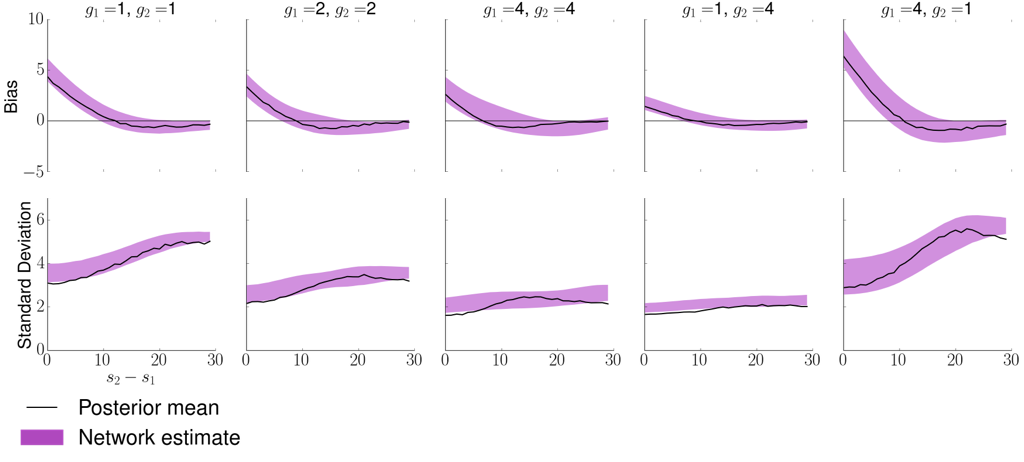
\includegraphics[width = \textwidth]{Fixed_Gains.png}
\caption{Error of the posterior mean and network estimates in the fixed gains condition. The pair of gains used for training the networks, computing the posterior and testing for each plot is listed above the plot.}
\end{figure}
\\
\\
In the real world, brains are confronted with a variable set of contrasts and so must attempt to ignore contrast in order to decode orientation from an input population like ours. Therefore, we now add a prior over gain which is uniform over all pairs of {1, 2, 4}. In the posterior computation, we now marginalize over this prior. For the network, we simply train the network using all combinations rather than just a single set of gains. We keep the training set at 270,000 trials and use 30,000 trials for each gain combination. We again split up the test performance by gain combination but since the networks were trained on all the gain combinations we use the same networks for all five plots. The standard deviations on the network error are computed over the performance of 400 networks. Again, the networks well approximate the posterior and seem to learn similar errors
\begin{figure}[h]
\centering
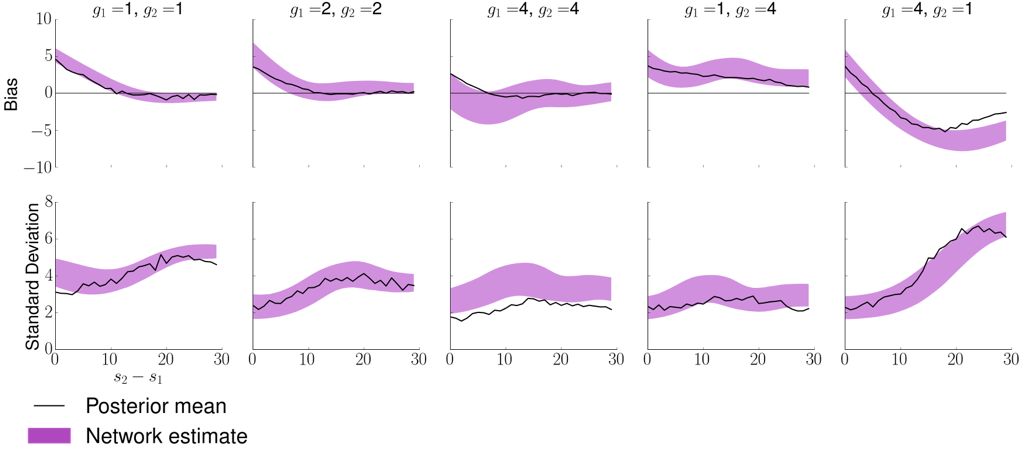
\includegraphics[width = \textwidth]{Variable_Gains.png}
\caption{Error of the posterior mean and network estimates in the variable gains condition. The pair of gains used for testing in each plot is listed above the plot. However, the same networks are used for all plots and in all plots the posterior mean marginalizes over gain.}
\end{figure}
\\
We wanted to check whether it was absolutely necessary to provide the network with all of the gain combinations. Since the network was trying to approximate a function, it is possible that it could interpolate, given some training data at the highest and lowest gain combinations. This generalization to unseen stimuli is a requirement for a brain in an uncertain world and the network's good performance on this task is surprising and suggests that it is truly approximating the posterior. The standard deviations on the network error are again computed over the performance of 400 networks. Like above, the same networks are used for all five plots. The posterior mean is exactly the same as in the variable gains condition since the problem statement hasn't changed.
\begin{figure}[h]
\centering
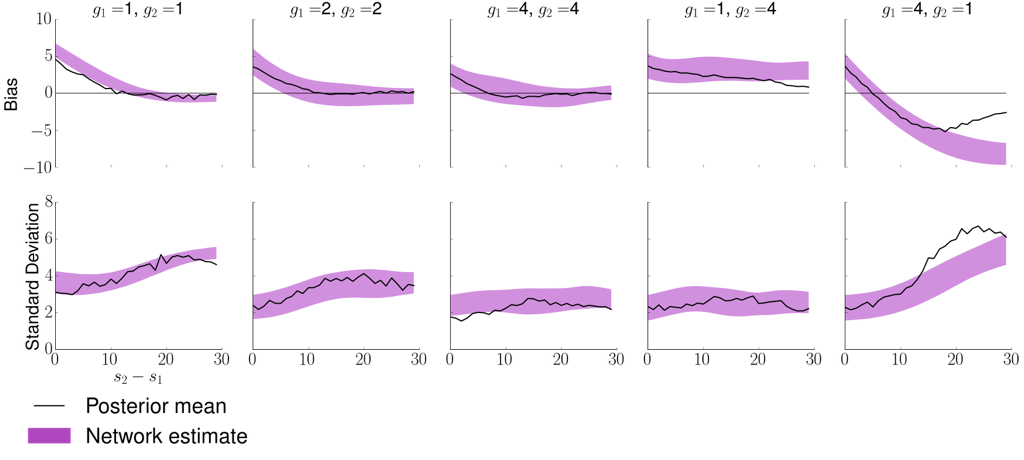
\includegraphics[width = \textwidth]{High-Low_Gains.png}
\caption{Error of the posterior mean and network estimates in the generalization condition. The pair of gains used for testing in each plot is listed above the plot. However, the same networks are used for all plots.}
\end{figure}
\\
Up until now we have been assuming that the estimation model knows that there are exactly two stimuli being encoded by the input population. However, this is rarely true in naturalistic cases. If the networks are providing a good approximation to the posterior they should be able to handle this unknown number of stimuli case as well. Using the network architecture that we have described above, it is difficult use a representation that allows for variable length outputs. Therefore, we used the following task to assess network performance in an uncertain number of stimuli scenario: on trials where there is only one stimulus, simply estimate that stimulus; on trials where there are two stimuli estimate the stimulus with the greatest contrast. For computing the posterior and for generating trials for training and testing, we used a discrete uniform prior over the number of stimuli. For the following discussion always called the higher contrast stimulus $s_{high}$ and set the gain of it's neural representation to 4. The lower contrast stimulus was $s_{low}$ and its gain was always 1. Because they are estimated according to their gains and not which stimulus is greater, we no longer need the triangular prior and $s_{high}$ and $s_{low}$ are both uniform over [-60, 60]. The network has the same architecture as above except it now has only one output node. We trained the network with the same number of training trials, learning algorithm and cost function as described above. For visualization, we fix $s_{high}$ at -30 and see how estimation varies as a function of the difference between $s_{high}$ and $s_{low}$. We again divide errors up into bias and standard deviation terms.
\begin{figure}[h]
\centering
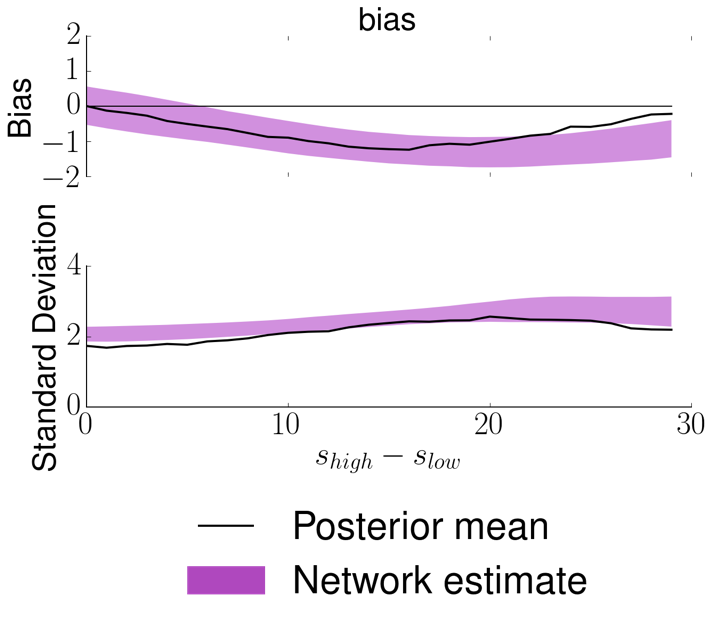
\includegraphics[width = .7\textwidth]{Single_Estimation.png}
\caption{Error of the posterior mean and network estimates in the variable number of stimuli condition.}
\end{figure}
\subsection{Precision Readout}
A natural question now is whether the network has not only learned to emulate the posterior mean when providing estimates of the stimuli but has also learned other features of the posterior distribution, despite not being trained directly. In particular, one behaviorally relevant quantity is the precision of the posterior. This quantity gives a measure of how uncertain the generated estimate which allows the agent using the estimates to make optimal decisions that rely on that estimate, according to Bayesian decision theory \cite{?}. And in fact, lots of evidence from the psychophysics literature suggests that people are able to well approximate this \cite{Qamar10122013}. For our purposes, we consider the network to have learned something if it is possible to easily decode the precision from the hidden unit representation.  We first tested this hypothesis using the hidden unit activations from the networks trained on all the gain combinations. In principle, these networks saw the widest range of posterior precisions during training so they would be the most likely to have learned a precision encoding. For the following plots, we used the network that we trained that achieved the lowest mean squared error. Perhaps the simplest method of decoding is to simply sum the activity of the hidden units, the idea being that the network should be more confident if there are higher hidden unit activations. However, this did not correlate at all with the trial-by-trial posterior precisions.  (r=-.1, 95\% CI [-0.23, 0.04]). 
\begin{figure}[h]
\centering
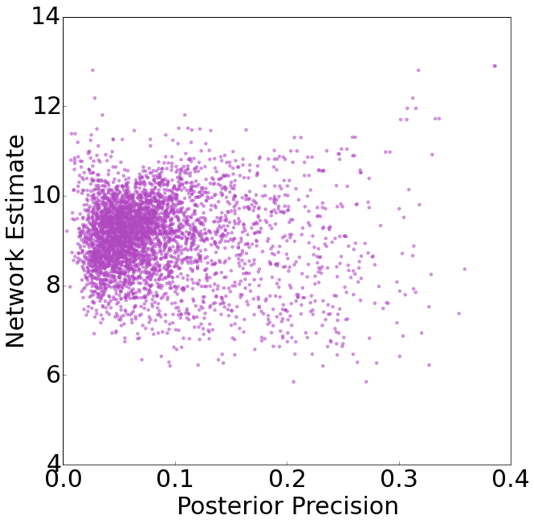
\includegraphics[width = .5\textwidth]{Sum_Precisions.png}
\caption{Correlation of the sum of the hidden unit activations and the posterior precision.}
\end{figure}
\\
We then tested whether a linear combination of the hidden unit activations would work for the precisions. This would still be a relatively simple readout: some downstream precision neuron would simply have to learn an appropriate set of weights in order to readout precision from the same set of neurons used for estimation. We are here asking whether we can well predict trial-by-trial precision with a linear regression on the hidden units. We kept the weights from the inputs to the hidden layer fixed and trained linear weights to predict precision using stochastic gradient descent as above. We used 133,000 trials to train the weights and then computed the correlation using 2,000 trials. This turned out to be highly correlated with the posterior precision (r=0.83,  95\% CI [0.78, 0.87]). 
\begin{figure}[h]
\centering
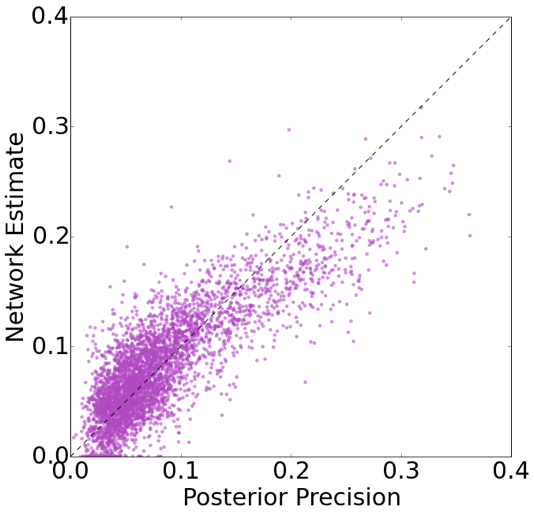
\includegraphics[width = .5\textwidth]{Linear_Combination_Precisions.png}
\caption{Correlation of trained linear combination of the hidden unit activations and the posterior precision.}
\end{figure}
\\
In fact, when we tried to do the same thing using the hidden layer from the networks trained only with single gain, correlations were not significantly lower (r=0.74, 95\% CI [0.67, 0.8]). We used a similar training procedure as described above.
\begin{figure}[h]
\centering
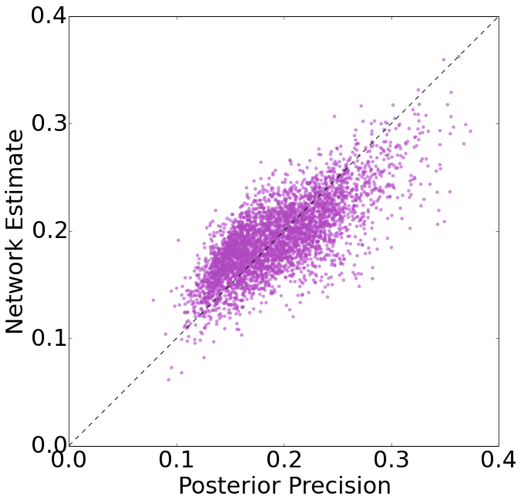
\includegraphics[width = .5\textwidth]{Linear_Fixed_Gains_Precisions.png}
\caption{Correlation of trained linear combination of the hidden unit activations from network only trained on a single gain combination and the posterior precision.}
\end{figure}
\\
So we have shown that it is easy to readout the precision from the hidden layer of the network that was trained only to solve the estimation task. However, it's possible that the network could have learned much better hidden units if it were only trying to estimate precision rather than also estimate the identities of the stimuli. In order to test what the best possible performance was using the functions available to our network, we trained three layer networks directly on precision. We used the same training procedure and parameters as described above. Here we achieved a high correlation (r=0.91, 95\% CI [0.88, 0.93]) but only slightly higher than that achieved by the linear combination. When the networks were trained to estimate the stimuli, they implicitly learned to linearize the precision in the hidden units simultaneously.
\begin{figure}[h]
\centering
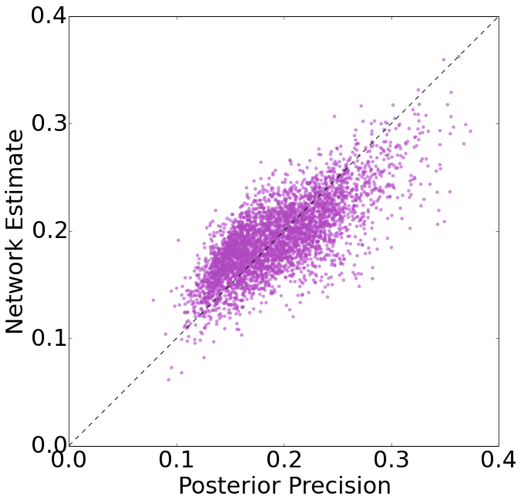
\includegraphics[width = .5\textwidth]{Linear_Fixed_Gains_Precisions.png}
\caption{Correlation of trained network estimates of precision and the posterior precision.}
\end{figure}

\section{Discussion}
We have demonstrated here that a simple three-layer network implementing only biologically plausible computations with relatively small numbers of hidden units can be easily trained to approximate the optimal Bayesian solution to the demixing problem. Here we have used orientation as a motivating example. However, this same computation could be used in any brain area involved in demixing which is why we used a generic prior over the stimuli. However, in future work, we would like to investigate how the use of more realistic priors (over specific types of stimuli) and heterogeneous input populations affect the performance of the network.
\\
In light of the universal function approximation theorem, this might not seem so surprising: we already knew that, given some arbitrary precision, there existed a number of neurons and a set of weights that could approximate this function to that precision. However, it wasn't a priori obvious that the demixing posterior should be possible to approximate with only 20 hidden units. In addition, a non-trivial result is that it is easy to learn the weights for these problems. This suggests that the loss surface for the posteriors that we investigated was relatively convex and should be easily learnable for other more biologically-plausible learning algorithms than backpropagation. In the future we would like to more generally map out the loss surface and investigate it's learnability by other algorithms. 
\\
Finally, the ability to linearly readout precision from the hidden units of the networks is a surprising result since this would not have been possible in other decoding schemes (such as \cite{Qamar10122013}). We would like to continue to investigate how exactly the hidden unit representation allows for this kind of readout. We would also like to understand and speak generally about what types of weights the network is learning. For example, are there always some neurons performing gain normalization, at least for the networks that need to marginalize over gain?
\\
Overall, these results demonstrate that neural networks are a promising direction for investigating how the brain could perform near-optimal inference in a biologically-plausible way.

\bibliography{abdnn}
\bibliographystyle{plain}

\end{document}